% 1977 年广东卷第 6 题：AE、AF 切圆 O 于 M、N，直径 EF 过圆心 O 且垂直于 AO，
% OM、ON 画虚线（按源卷第 3 页布局）
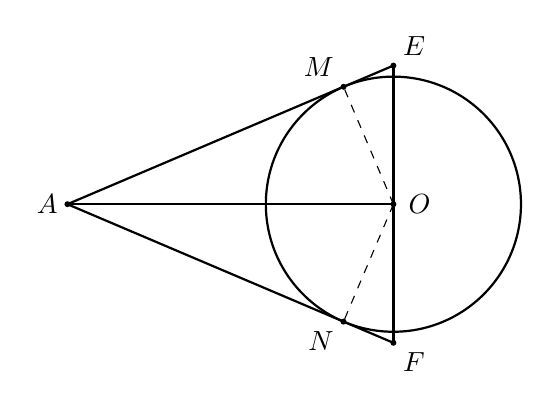
\begin{tikzpicture}[scale=0.9]
  \draw[thick] (0,0) circle (1.8);
  \coordinate (O) at (0,0);
  \coordinate (A) at (-4.6,0);
  \coordinate (M) at (-0.704,1.657);
  \coordinate (N) at (-0.704,-1.657);
  \coordinate (E) at (0,1.956);
  \coordinate (F) at (0,-1.956);
  \draw[thick] (A) -- (E);
  \draw[thick] (A) -- (F);
  \draw[thick] (A) -- (O);
  \draw[thick] (E) -- (F);
  \draw[dashed] (O) -- (M);
  \draw[dashed] (O) -- (N);
  \fill (O) circle (1.2pt) node[right=2pt] {$O$};
  \fill (A) circle (1.2pt) node[left] {$A$};
  \fill (M) circle (1.2pt) node[above left] {$M$};
  \fill (N) circle (1.2pt) node[below left] {$N$};
  \fill (E) circle (1.2pt) node[above right] {$E$};
  \fill (F) circle (1.2pt) node[below right] {$F$};
\end{tikzpicture}
